\documentclass[10pt]{article}
\usepackage[utf8]{inputenc}
\usepackage[english]{babel}
\usepackage{graphicx}
\usepackage{amsmath}
\usepackage{amssymb}
\usepackage{hyperref}
\usepackage{tikz}
\usetikzlibrary{arrows,decorations.pathmorphing,decorations.markings,backgrounds,positioning,fit,topaths,shapes,patterns,calc}

\newcommand{\dd}{\mathrm{d}}

\renewcommand{\vec}[1]{\mathbf{#1}}
\newcommand{\ve}{\vec{e}}
\newcommand{\vi}{\vec{i}}
\newcommand{\vn}{\vec{n}}
\newcommand{\vx}{\vec{x}}

\begin{document}

\title{Memristor mathematical model, ver. 1.0}
\author{https://github.com/eugnsp/memristor}
\maketitle

% ================================================================================
\section*{Equations, their discretization and algorithms}

Note: in what follows atomic units are used.

% --------------------------------------------------------------------------------
\section*{Heat equation}

The heat equation for the lattice temperature~$T(\vx)$ is
\begin{equation}
-\nabla \cdot [ c(\vx) \nabla T(\vx) ] = s(\vx),
\end{equation}
where $c(\vx)$ is the thermal conductivity, and $s(\vx)$ is the volume heat
density of the source.

In the cylindrical coordinates this equation for~$T(\vx) = T(r, z)$ takes the form:
\begin{equation}
\label{eq:heat_equation_rz}
- \frac{\partial}{\partial r} \left[ c(r, z) \frac{\partial T}{\partial r} \right]
- \frac{c(r, z)}{r} \frac{\partial T}{\partial r}
- \frac{\partial}{\partial z} \left[ c(r, z) \frac{\partial T}{\partial z} \right]
= s(r, z).
\end{equation}

The structure of the heat source term is
\begin{equation}
s(r, z) = \frac{\theta [ r_0(z) - r ]}{\pi r_0(z)^2} s(z),
\end{equation}
where $r_0(z)$~is the source radius, and $s(z)$~is its linear density. It is
tempting to approximate the source with a delta-functional one
\begin{equation}
s(r, z) = \delta (\pi r^2) s(z) = \frac{\delta(r)}{2\pi r} s(z).
\end{equation}
However, the solution of~\eqref{eq:heat_equation_rz} is singular at~$r = 0$:
$T(r) \sim \ln(r)$. Hence, finite~$r_0$ should be retained. For simplicity we
assume $r_0 := \{ \mathsf{heat\_source\_radius} \}$ to be independent of~$z$.
Due to the logarithmic divergence the solution is very sensitive to the value
of $r_0$ for $r < r_0$.

The heat is produced due to the Joule heating:
\begin{equation}
\label{eq:heat_joule_source}
s(z) = I^2 r_c(z),
\end{equation}
where $I$ is the total current, and $r_c(z)$ is the linear resistivity of the core.

The thermal conductivity is assumed to be uniform in the whole system:
\begin{equation}
c(r, z) = c := \{ \mathsf{thermal\_conductivity} \}.
\end{equation}

% ................................................................................
\subsection*{Boundary conditions}

The uniform Dirichlet boundary condition is assumed at the outer surface:
\begin{equation}
T(\vx)\vert_\Gamma = T_0 := \{ \mathsf{temperature} \}.
\end{equation}

This condition translates into the following condition in the cylindrical
coordinates:
\begin{equation}
T(r, z)\vert_\Gamma = T_0.
\end{equation}
along with the compatibility condition at $r = 0$
\begin{equation}
\label{eq:temp_compatibility_bc}
\frac{\partial T(r, z)}{\partial r} \bigg\vert_{\Gamma_0} = 0, \quad
\end{equation}

% ................................................................................
\subsection*{Discretization}

Multiplying eq.~\eqref{eq:heat_equation_rz} by~$r$, we obtain
\begin{equation}
- r \nabla \cdot ( c \nabla T ) - c \frac{\partial T}{\partial r}
= \frac{I^2}{\pi r_0^2} \theta(r_0 - r) r_c, \quad
\nabla = (\partial_r, \partial_z).
\end{equation}

After multiplication by a test function~$\chi(r, z)$ and integration by parts
we get
\begin{multline}
- \int_\Omega r \chi \nabla \cdot ( c \nabla T )
- \int_\Omega \chi c \frac{\partial T}{\partial r}
%
= \int_\Omega c [ \nabla ( r \chi ) \cdot \nabla T ]
- \int_\Gamma r \chi c [ \nabla T \cdot \hat{\vn} ]
- \int_\Omega \chi c \frac{\partial T}{\partial r} = \\
%
= \int_\Omega r c [ \nabla \chi \cdot \nabla T ]
- \int_\Gamma r \chi c [ \nabla T \cdot \hat\vn ]
%
= \frac{I^2}{\pi r_0^2} \int_\Omega r \chi \theta(r_0 - r) r_c.
\end{multline}

The space of test functions is chosen such that $\chi$ vanishs at the Diriclet
boundary. Then due to the compatibility condition~\eqref{eq:temp_compatibility_bc}
the boundary term drops out:
\begin{equation}
\int_\Omega r c [ \nabla \chi \cdot \nabla T ]
= \frac{I^2}{\pi r_0^2} \int_\Omega r \chi \theta(r_0 - r) r_c.
\end{equation}

To account for non-zero Dirichlet boundary conditions, we make a substitution
$T \to T + T_b$, where $T$ now has zero boundary conditions, and $T_b$ is an
arbitrary function such that $T_b |_\Gamma = T_0$:
\begin{equation}
\int_\Omega r c [ \nabla \chi \cdot \nabla T ]
= \frac{I^2}{\pi r_0^2} \int_\Omega r \chi \theta(r_0 - r) r_c
- \int_\Omega r c [ \nabla \chi \cdot \nabla T_b ]
\end{equation}

Expanding $T = \sum_j T_j \chi_j$ over basis functions~$\chi_i$ and using the
Galerkin's method, we get the discrete system for the $T_j$ coefficients:
\begin{equation}
\sum_j S_{ij} T_j = b_i,
\end{equation}
where
\begin{equation}
S_{ij} = \int_\Omega r c [ \nabla\chi_i \cdot \nabla\chi_j ], \quad
%
b_i = \frac{I^2}{\pi r_0^2} \int_\Omega r \chi_i \theta(r_0 - r) r_c
- \int_\Omega r c [ \nabla\chi_i \cdot \nabla T_b ].
\end{equation}

% --------------------------------------------------------------------------------
\section*{Poisson's equation}

The Poisson's (Laplace's) equation for the electrostatic potential~$\phi(\vx)$
with zero charge density is
\begin{equation}
\nabla[ \epsilon(\vx) \nabla \phi(\vx) ] = 0.
\end{equation}

\textbf{Boundary conditions}

\begin{figure}[!h]
\centering
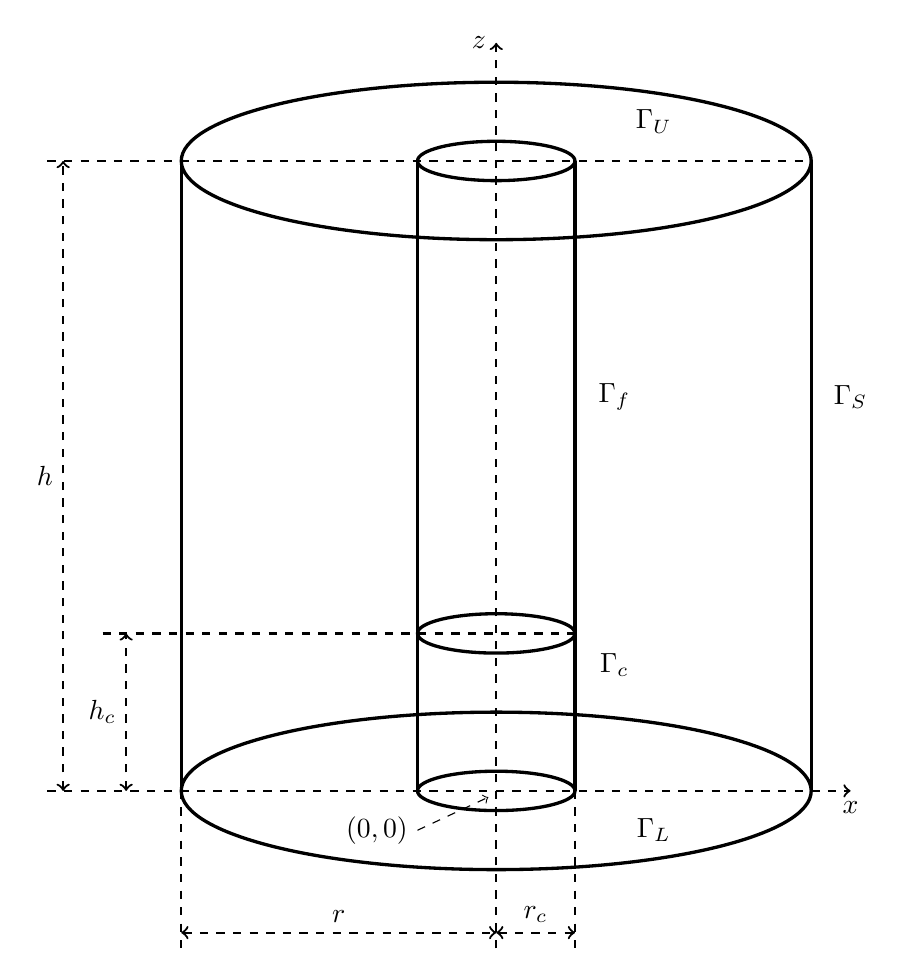
\begin{tikzpicture}
	\draw[very thick] (0, 0) ellipse [x radius = 4, y radius = 1];
	\draw[very thick] (0, 8) ellipse [x radius = 4, y radius = 1];
	\draw[very thick] (-4, 0) -- (-4, 8);
	\draw[very thick] (4, 0) -- (4, 8);

	\draw[very thick] (0, 0) ellipse [x radius = 1, y radius = .25];
	\draw[very thick] (0, 8) ellipse [x radius = 1, y radius = .25];
	\draw[very thick] (0, 2) ellipse [x radius = 1, y radius = .25];
	\draw[very thick] (-1, 0) -- (-1, 8);
	\draw[very thick] (1, 0) -- (1, 8);

	\draw[->,thick,dashed] (-5.7, 0) -- (4.5, 0) node[below] {$x$};
	\draw[thick,dashed] (-5, 2) -- (1, 2);
	\draw[thick,dashed] (-5.7, 8) -- (4, 8);

	\draw[<->,thick,dashed] (-5.5, 0) -- (-5.5, 8) node[midway,left] {$h$};
	\draw[<->,thick,dashed] (-4.7, 0) -- (-4.7, 2) node[midway,left] {$h_c$};

	\draw[->,thick,dashed] (0, -2) -- (0, 9.5) node[left] {$z$};
	\draw[thick,dashed] (-4, 0) -- (-4, -2);
	\draw[thick,dashed] (1, 0) -- (1, -2);

	\draw[<->,thick,dashed] (-4, -1.8) -- (0, -1.8) node[midway,above] {$r$};
	\draw[<->,thick,dashed] (0, -1.8) -- (1, -1.8) node[midway,above] {$r_c$};

	\draw (2, -.5) node {$\Gamma_L$};
	\draw (2, 8.5) node {$\Gamma_U$};
	\draw (1.5, 1.6) node {$\Gamma_c$};
	\draw (1.5, 5) node {$\Gamma_f$};
	\draw (4.5, 5) node {$\Gamma_S$};

	\draw[->,dashed] (-1, -.5) node[below,left] {$(0, 0)$} -- (-.1, -.08);

\end{tikzpicture}
\caption{Boundary conditions for the Poisson equation.}
\end{figure}

Dirichlet boundary conditions are used everywhere:
\begin{equation}
\phi(\vx)\vert_{\Gamma_L \cup \Gamma_c} = 1, \quad \phi(\vx)\vert_{\Gamma_R} = 0, \quad
\phi(\vx)\vert_{\Gamma_S} = 1 - \frac{z}{h}, \quad \phi(\vx)\vert_{\Gamma_f} = 1 - \frac{R(h_c, z)}{R(h_c, h)},
\end{equation}
where $R(z_1, z_2)$ is the resistance of the filament between points $z_1$ and $z_2$.

%At the side surface, $\partial\Omega_S$, zero Neumann boundary condition:
%\begin{equation}
%\partial_n \phi(\vx)\vert_{\partial\Omega_S} = E_n(\vx)\vert_{\partial\Omega_S} = 0.
%\end{equation}

%These physical boundary conditions translate into the mathematical ones:
%\begin{equation}
%\phi(r, z)\vert_{z = 0} = \phi_S, \quad \phi(r, z)\vert_{z = h} = \phi_D, \quad \frac{\partial \phi(r, z)}{\partial r}\bigg\vert_{r = R} = 0.
%\end{equation}

%At $r = 0$ the following compatibility condition holds for any continuous function:
%\begin{equation}
%\frac{\partial \phi(r = R, z)}{\partial r}\bigg\vert_{r = 0} = 0.
%\end{equation}

% --------------------------------------------------------------------------------
\section*{Kinetic Monte-Carlo method}

The distribution of vacancies is described by the occupation numbers $v_\vi$,
which can only be 0 (no vacancy) or 1 (single vacancy), with indices $\vi$
defined on the discrete 3D uniform grid $\mathcal{G}$,
\begin{equation}
\mathcal{G} = \{ \vi = (i, j, k) \ | \ \vx_\vi \in \overline\Omega_D \},
\end{equation}
where $\vx_\vi$ are the coordinates of the site~$\vi$. The grid spacing equals
$\delta := \{ \mathsf{grid\_delta} \}$.

It is assumed that vacancies hop only between nearest-neighbour sites. Each site
(except for boundary ones) has six nearest neighbours. The rate (probability per
unit time) of hopping is
\begin{equation}
\Gamma_{\vi \to \vi'} = v_\vi (1 - v_{\vi'}) w_0
\exp \left\{
	-\frac{E_{\mathrm{ac}} + [U(\vx_{\vi'}) - U(\vx_\vi)]}
	{T[(\vx_\vi + \vx_{\vi'}) / 2]}
\right\}, \quad U(\vx) = q \phi(\vx),
\end{equation}
where $w_0 := \{ \mathsf{debye\_frequency} \}$ is the Debye frequency, $T(\vx)$
is the temperature, $\phi(\vx)$ is the electrostatic potential, and $q = e > 0$
is the O-vacancy charge. The pre-factor $v_\vi (1 - v_{\vi'})$ takes into account
that the hopping is possible only if the source site is occupied ($v_\vi = 1$)
and the destination one is empty ($v_{\vi'} = 0$).

% ................................................................................
\subsection*{Initial conditions}

Initially all vacancies are distributed uniformly randomly over~$\mathcal{G}$
with the filling factor $\rho := \{ \mathsf{initial\_filling} \}$,
$0 < \rho < 1$, such that the total number of vacancies is
$\lfloor \rho N_{\mathcal{G}} \rfloor$, where $N_{\mathcal{G}}$ is the total
number of sites in~$\mathcal{G}$.

% ................................................................................
\subsection*{Boundary conditions}

TODO. If the source or final cite lies outside the domain, the hopping probabilities are determined by the boundary conditions.

% ................................................................................
\subsection*{Algorithm}

Variable step size method is used for Monte-Carlo simulation. The following
algorithm is used.

\begin{enumerate}
\item \label{alg:monte_carlo_events} Identify all possible events and compute
their rates $\Gamma_k = \Gamma_{\vi \to \vi'}$.

\item Compute probabilities of all events: $P_k = \Gamma_k / \Gamma$, where
$\Gamma = \sum_k \Gamma_k$ is the total rate. Select the next event randomly
according to this probability distribution.

\item Compute the time step: $\Delta t_i = -\ln u / \Gamma$, where where $u$
is a uniform random number in the range~$(0, 1)$.

\item Check if the total simulation duration $\Delta t = \sum_i \Delta t_i$
and/or the number of steps exceed the given limits. Abort, if they do.

\item Go to step \ref{alg:monte_carlo_events}.
\end{enumerate}

%Next event is chosen from

% \subsection{Electric Conductivity}
% \label{sec:ElectricConductivity}

% Electric conductivity of the filamentary media, as well as the same of the rest of the dielectric media with the vacancies are to be discussed.

% For the metallic granule the value of $\sigma_G = 10^7$ (1/(Ohm*m) is taken.

% \subsection{Heat source}

% \begin{figure}[!h]
% \centering
% \begin{tikzpicture}
% 	\draw[very thick] (0, 0) ellipse [x radius = 4, y radius = 1];
% 	\draw[very thick] (0, 11) ellipse [x radius = 4, y radius = 1];
% 	\draw[very thick] (-4, 0) -- (-4, 11);
% 	\draw[very thick] (4, 0) -- (4, 11);

% 	\draw[very thick] (0, 8) ellipse [x radius = 1, y radius = .25];
% 	\draw[very thick] (0, 2) ellipse [x radius = 1, y radius = .25];
% 	\draw[very thick] (-1, 2) -- (-1, 8);
% 	\draw[very thick] (1, 2) -- (1, 8);

% 	\draw[thick,dashed] (-5.7, 0) -- (4, 0);
% 	\draw[thick,dashed] (-5, 2) -- (1, 2);
% 	\draw[thick,dashed] (-5.7, 8) -- (1, 8);
% 	\draw[thick,dashed] (-5.7, 11) -- (4, 11);

% 	\draw[<->,thick,dashed] (-5.5, 0) -- (-5.5, 8) node[midway,left] {$h$};
% 	\draw[<->,thick,dashed] (-4.7, 0) -- (-4.7, 2) node[midway,left] {$h_c$};
% 	\draw[<->,thick,dashed] (-5.5, 8) -- (-5.5, 11) node[midway,left] {$h_t$};

% 	\draw[thick,dashed] (0, 12) -- (0, -2);
% 	\draw[thick,dashed] (-4, 0) -- (-4, -2);
% 	\draw[thick,dashed] (1, 2) -- (1, -2);

% 	\draw[<->,thick,dashed] (-4, -1.8) -- (0, -1.8) node[midway,above] {$r$};
% 	\draw[<->,thick,dashed] (0, -1.8) -- (1, -1.8) node[midway,above] {$r_c$};

% 	\draw (0.5, 5) node {$s(\vx)$};

% \end{tikzpicture}
% \caption{Heat source for the heat equation.}
% \end{figure}

% The heat source~$s(\vx)$ is given by
% \begin{equation}
% s(\vx) = \begin{cases}
% P(z), & x^2 + y^2 \leq R_f(z)\ \text{and}\ h_c < z < h, \\
% 0, & \text{otherwise},
% \end{cases}
% \end{equation}
% where $P(z)$ is Joule heat source and $R_f(z)$ is the filament radius.

% \section{Calculation of resistance}

% Firstly, one calculates the coordinate of the end of the filament ($z_2$) and its radia (as function of $z$).

% The radia array $r(z)$ is calculated as the following.
% For every taken $z$ one calculates the fraction of nodes, occupied by the vacancies, in the layer (excluding the nodes, occupied by the granules).
% If the fraction is larger, than some value $x_c$ (here $x_c=0.25$), then the radius is increased by one lattice period, (i.e. $r(i+1)$ = $r(i)$ + $a$,
% where $a$ is the lattice period?)(-V.)and the calculation is repeated. That is done, until calculated fraction is smaller, than $x_c$, twice during the
% calculation

% The length of the filament is calculated from the coordinate of the beginning of the filament $z_1$ (here $z_1=30$ layers $=30a$). $z_2$ is the coordinate just before the second zero $r(z)$ since $z_1$ (i.e., a single gap in the filament is allowed). (The same difficulty, concerning $L_v >a$, as above)(V.)

% Then one calculates the resistance layer by layer.
% If there is granule in the layer $z_i$, then its resistance is taken as
% \begin{equation}
% R_{\text{gran}}(z_i)=\rho_{\text{gran}}\frac{\delta z}{S_{\text{gran}}(z_i)},
% \end{equation}
% where $\rho_{\text{gran}}=0.096$ $\Omega$*mm$^2$/m is the granule material resistivity, $\delta z=a=0.25$ nm is the width of the layer, and $S=\pi r_{\text{gran}}^2(z_i)$ is the actual filament area. If there is also filament in the layer, its resistance is
% \begin{equation}
% R_{\text{fil}}(z_i)=\rho_{\text{fil}}\left(1+\frac{\alpha}{2(r_{\text{fil}}-r_{\text{gran}})}\right)\frac{\delta z}{S_{\text{fil}}(z_i)},
% \end{equation}

% \begin{equation}
% 	R_{\text{fil}}(z_i)=\rho_{\text{fil}}\frac{\delta z}{S_{\text{fil}}(z_i)[1-(r_{\text{gran}}/r_{\text{fil}})^2]}
% \end{equation}
% where $\rho_{\text{fil}}=2.4\times10^{-2}$ $\Omega$*mm$^2$/m, $\alpha=10.5$ nm.
% Then the total resistance is
% \begin{equation}
% R(z_i)=\frac{R_{\text{fil}}R_{\text{gran}}}{R_{\text{fil}}+R_{\text{gran}}}.
% \end{equation}

% If there is no filament and granule, the resistance is taken as:
% \begin{equation}
% R(z_i)=\delta z\times10^7\times5\times10^{-4}/\pi,
% \end{equation}
% where $\delta z$ is taken in nm.

% Finally, the resistance of the element is just
% \begin{equation}
% R=\sum_i R(z_i).
% \end{equation}

% --------------------------------------------------------------------------------
\section*{Resistance and potential distribution}

% --------------------------------------------------------------------------------
\section*{Interpolation between meshes}

% --------------------------------------------------------------------------------
\section*{Device simulation algorithm}

The device simulation proceeds according to the following algorithm:

\begin{enumerate}
\item \textbf{Initialization.} Read the mesh for the heat equations from the
external file; create the mesh for the Poisson equation; initialize the
finite-element solvers; initialize the Monte-Carlo solver; generate the initial
distribution of O-vacancies.

\item Set bias voltage to zero: $V \gets 0$; set bias voltage sweep direction to
``forward'': $\xi \gets +1$.

\item \label{alg:main_compute_shape} \textbf{Main loop.} Compute the filament
shape.

\item Compute the linear resistance $r_c(z)$; compute
the total current~$I$; compute the linear heat source density $I^2 r_c(z)$;
compute the Poisson equation boundary condition $\phi(0, z)$.

\item Solve the heat equation for $T(r, z)$; solve the Poisson equation for
$\phi(r, z)$; interpolate to the Monte-Carlo grid to obtain $T(\vx_i)$ and
$\phi(\vx_i)$.

\item Estimate the duration $\langle \Delta t \rangle$ of a single Monte-Carlo
step. If it is larger than the minimum Monte-Carlo step duration
$\langle \Delta t \rangle_{\min} := \{ \mathsf{min\_step\_duration} \}$, set
time step: $\Delta t \gets \overline{\Delta t}_{\min}$, and go to step
\ref{alg:main_update_bias} (skip Monte-Carlo simulation).

\item Run the Monte-Carlo simulation for $n := \{ \mathsf{steps\_per\_round} \}$
steps; compute the elapsed time $\Delta t$.

\item \label{alg:main_update_bias} Update bias voltage:
$V \gets V + \xi s \Delta t$, where $s := \{ \mathsf{bias\_sweep\_rate} \}$
is the bias voltage sweep rate.

\item Go to step \ref{alg:main_compute_shape}.
\end{enumerate}


\end{document}
